\documentclass{cidr-2019}

\usepackage{float}
\setcounter{topnumber}{10}
\def\topfraction{.9}
\setcounter{bottomnumber}{10}
\def\bottomfraction{.9}
\setcounter{totalnumber}{10}
\def\textfraction{0}
\def\floatpagefraction{.9}
\setcounter{dbltopnumber}{10}
\def\dbltopfraction{.9}
\def\dblfloatpagefraction{.9}


\begin{document}

\title{Beyond Design Continuums}

\numberofauthors{3}
\author{
\alignauthor
Mali Akmanalp\\
       \affaddr{Harvard University}\\
       \email{mea590@g.harvard.edu}
\alignauthor
A. Sophie Hilgard\\
       \affaddr{Harvard University}\\
       \email{ash798@g.harvard.edu}
\alignauthor Andrew Ross\\
       \affaddr{Harvard University}\\
       \email{andrew\_ross@g.harvard.edu}}

\date{\today}

\maketitle

\section{Beyond Design Continuums}

%Design continuums are higher-order performance models where the inputs are
%design decisions for a data structure, and the outputs are performance
%characteristics. Much like other types of models (e.g. economic models), they
%start with a set of assumptions and describe the variation in behavior as the
%input variables change.

%continuous space...

Creating design continuums can become non-trivial when we add additional knobs,
or bring simpler continuums together to build a more complex continuum.

\textbf{Complex parameter spaces:} In many cases the knobs might display a high
level of sensitivity to the values of other knobs. This kind of complex
interaction can make the manual construction of a proper design continuum
intractable.

Consider the critical design decision of how much memory to allocate to a cache
in an LSM-tree. Since we have a fixed amount of main memory, the size of the
cache must interact in multiple ways with the sizes of other memory
allocations.

Increasing the size of the cache requires a reduction in the size of the
buffer and bloom filters, but what is the best way to distribute the
reduction among the two? If we choose to take away from the size of the
buffer, we might assume that more queries will end up touching the lower and
slower levels of the LSM-tree. Is this penalty offset by the larger cache? This
depends on the hit rate of the cache, which ultimately depends on the query
workload.

If we have a workload where a small set of keys dominates the majority of
queries, then perhaps the improvement from cache hits will dominate performance
characteristics, and we will get an overall improvement in performance.
Alternatively, if we have a workload where the hot set of keys is larger than
the cache or perhaps even main memory, then we might find that the strategy
suddenly turns into a bad one - e.g. a relatively small proportion of queries
that cause a cache miss and hit disk might be enough to sink overall
performance because by reducing the space allocated to bloom filters we've made
them highly inaccurate, meaning that we'll now have to scan most layers fully. 

If we had instead decided in the beginning to remove more from the bloom
filters rather than the buffer, we'd encounter a different set of dilemmas in
the decision making process. On top of this, was increasing the size of the
buffer a good decision in the first place? We would need yet another set of
criteria to be able to make that determination.

\textbf{Non-continuous parameter spaces:} we might have design knobs that are
not smooth and continuous, but are made of many discrete options.

\textbf{Complex workloads:} In real world scenarios we might e.g. find that the
hot set of keys is not static but changes over time, affecting performance with
it \cite{characterizing-memcached}.

For only a few parameters, we can end up with a situation where even hand-wavy
intuition on tradeoffs becomes complicated. Knowing the exact parameters or the
exact tipping points in which certain strategies become better or worse is yet
harder. At each turn, we encounter more "it depends" scenarios.

\subsection{A solution: Stochastic Gradient Descent}

We see a path forward by combining machine learning techniques with design
continuum knowledge to create solutions that approach the optimal design for a
broader set of design decisions. The problem, to us, seems akin to training a
machine learning model:

\textbf{The cost function} that we're minimizing is the I/O access cost,
derived from the design continuum.

\textbf{The goal} is to minimize the cost function, i.e. find the parameters
that provide the lowest I/O cost for the given set of queries.

\textbf{The parameters} are the cache size, the buffer size and the bloom
filter size.

\textbf{The parameter space} is only a subset of 3D space, because total memory
is constrained. For example, if we wanted to increase both the cache size and
the buffer size we would have to decrease the bloom filter size. This
parameter space is described by a 2-simplex.

\textbf{The gradient functions} are the estimated I/O savings if we increase
the memory by N bits for any single component. Following the gradients, one
would expect to end up in a minima. While deriving these analytically is
difficult, we come up with reasonable estimates using the design continuum cost
formulas.

\textbf {The dataset} we're training the model on is a workload, i.e. a set of
queries. We automatically generate ours from probabilistic models, but one
could also use traces of real systems, or perhaps a combination of both.

\subsection{Stochastic Workloads}

To avoid overfitting to a particular set of queries, we define some workload
classes as configurable probabilistic models. We can then generate an ordered
sequence of reads or updates (i.e. a workload) from any of these. We include
more complex, time-varying workloads (inspired by
\cite{characterizing-memcached} and \cite{linkbench}) that attempt to mimic
realistic settings.

For all the workloads, when we draw a particular key for the first time we
will insert it into the database as a write, and subsequently we will either
look it up or update it with probability $w$.

\textbf{Uniform} queries will be drawn uniformly from a set of $K$ keys. This is
often one in which the cache is unhelpful, but in practice may be unrealistic.
Nevertheless, this is the scenario that many analyses assume.

\textbf{Round-Robin} queries are drawn deterministically using $k_i = (i \mod
K)$, i.e. we iteratively draw each key in sequence, then repeat.
This is represents another pathological scenario for a cache: a key has been
recently written or read is actually a contraindication we will access it
again.

\textbf{80-20} queries (considered in \cite{monkey}) are drawn such that 20\%
of the most recently inserted keys constitute 80\% of the lookups. This is a
simple model to observe the effects of skew.

\textbf{Zipf} queries are distributed according to a zeta distribution, with a
parameter $s$ which describes the skewness. Zipf-distributed queries are
considered in \cite{art} as another simple proxy for realistically skewed
queries.

\textbf{Discover-Decay} queries are distributed according to the following
stochastic process, inspired by the Chinese Restaurant process \cite{crp} but
with time decay: with every passing time step, we draw a number of reads $n_r$,
writes $n_w$, and updates $n_u$ assuming queries arrive according to Poisson
processes with configurable rates: \[
\begin{split}
  n_r & \sim \textrm{Pois}(\lambda_r) \\
  n_w & \sim \textrm{Pois}(\lambda_w) \\
  n_u & \sim \textrm{Pois}(\lambda_u)
\end{split}
\]
Once we've drawn our $n_w$ new keys $k_i$, we assign them an initial popularity
$$
\theta_{i} \sim \textrm{Beta}(a_\theta,b_\theta)
$$
\noindent with a random decay rate
$$
\gamma_i \sim \textrm{Beta}(a_\gamma,b_\gamma),
$$
which is the factor by which they exponentially decay each subsequent time
step. At any time $t$, the popularity of each key is given by $p(k_i,t) \propto
\theta_i\gamma_i^{t-t_i}$, where $t_i$ is when the key was inserted. We use
these time-dependent popularities to draw each of our $n_r$ reads and $n_u$
updates from $\textrm{Mult}(\{p(k_i,t)\})$.

\textbf{Periodic Decay} workloads are a simple modification of the
Discover-Decay model where $p(k_i,t)$ now depends not only on the decay rate
$\gamma_i$ but also on a periodic function of the key's age $t-t_i$.  To mimic
the combination of exponential decay and sharp periodic peaking we see in
\cite{characterizing-memcached}, we multiply $\theta_i\gamma_i^{t-t_i}$ by an
inverse cycloid function with period $T$, clamped from 0 to 1, and taken to a
configurable power (to make the cusps sharper or duller) that we call the
cycloid's \texttt{cuspity}.

Examples of these workloads can be seen in Figure \ref{fig:workloads} in
Appendix \ref{workloads}.

\subsection{Modeling}

We derive equations for the number of disk accesses saved by adding N bits more
space to a component. We store simple O(1) space statistics (e.g. number of
queries, number of accesses for each bloom filter, number of times a key was
found in a layer) to get easy to compute and reasonable estimates for these.
These loosely follow the general form:

\begin{align*}
    &\Delta accesses = \widehat{hit\_rate}\cdot \Delta{entries} \cdot\widehat{miss\_cost}
\end{align*}

More specifically:

\begin{align*}
    &\Delta cache = \widehat{last\_slot\_hits} \cdot \Delta{entries} \cdot  \widehat{avg\_cost\_of\_miss} \\
    &\Delta buffer = \sum_{l\in L} \widehat{accesses_{l}} \cdot \frac{dM \cdot {layer\_ratio}}{Mlayer_{l}} \cdot \widehat{avg\_cost\_of\_miss_{l}}\\
    &\Delta bloom = \sum_{l\in L} \widehat{accesses_{l}} \cdot alloc(l, m+dM) \cdot \widehat{\Delta false\_pos\_rate_{l}}\\
\end{align*}

For full derivations, refer to Appendix \ref{modeling}.

\subsection{Gradient Descent}

Results for basic workloads can be seen in Figure \ref{fig:basicquiv}. To
display our results, we introduce a specific plot that shows the workload, our
estimated gradients at each point, our estimated best configurations, the
actual performance across the whole parameter space and the actual optimal
configuration.

\textbf{The triangle} shows the parameter space. Each coordinate within the
space represents an LSM tree with a particular combination of these parameters.
Perpendicular distance from the edge opposite a corner represents the value for
that corner's parameter, e.g. a coordinate in the very center represents an
equal allocation of all three parameters and a coordinate at a corner
represents allocating everything to only that parameter.

\textbf{The arrows} represent our estimated gradient around that coordinate
i.e. given the current set of parameters, which direction our I/O savings model
says you should move to get a better total I/O cost.

\textbf{The orange dots} signify the parameters we predict will have the
minimum I/O cost.  One can start the gradient descent process from any given
initial point. We test our method with every possible initial point to ensure
that it consistently yields good results, which is why there is more than one
prediction.

\textbf{The blue-red shading} represents actual I/O cost for each parameter
combination, generated by exhaustively running queries from the workload on an
LSM tree simulator.

\textbf{The yellow dot} represents the lowest actual minimum I/O cost
determined experimentally, and therefore the optimal allocation of parameters -
our target.

The gradient descent process works as follows:

\begin{itemize}
\setlength{\itemsep}{0pt}
\setlength{\parskip}{0pt}
\setlength{\parsep}{0pt}
\item Ignoring the shading, start at any random initial parameters. Follow the
    arrows until you either hit the edge of the parameter space or hit a point
        where there are no outward arrows from your current location.
\item To evaluate our results, one can look at the plot and should check to see
    that the predicted minima (orange dots) are nearby the actual minimum
        (yellow dot), or failing that on a grid coordinate with similar IO cost
        (judged by the blue-red shading).
\end{itemize}

Results for basic workloads can be seen in Figure \ref{fig:basicquiv}. For each
workload, we provide results for both the even and the Monkey bloom filter
allocation schemes.

The uniform workload provides a baseline workload to compare other results to.
The round-robin workload provides an example of a canonical workload that
thrashes the cache to the point where it is useless, and indeed our
recommendation is to allocate no space to the cache. Discontinuities in the
number of layers as we vary the buffer size makes the optimization
non-convex, but Monkey improves both absolute performance and convexity.

\begin{figure}[!htb]
\begin{center}
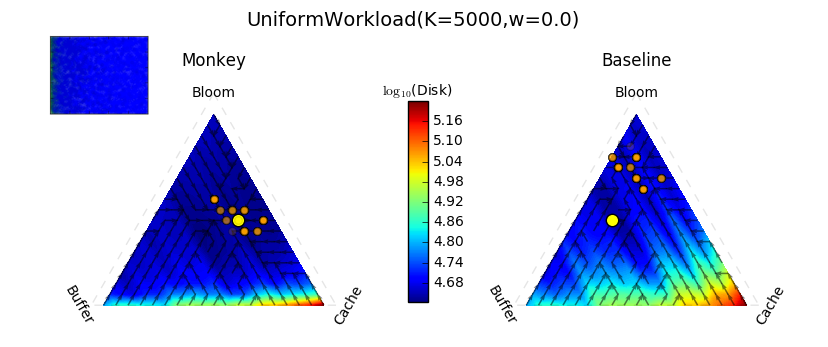
\includegraphics[width=0.5\textwidth]{uniformquiv1.png}
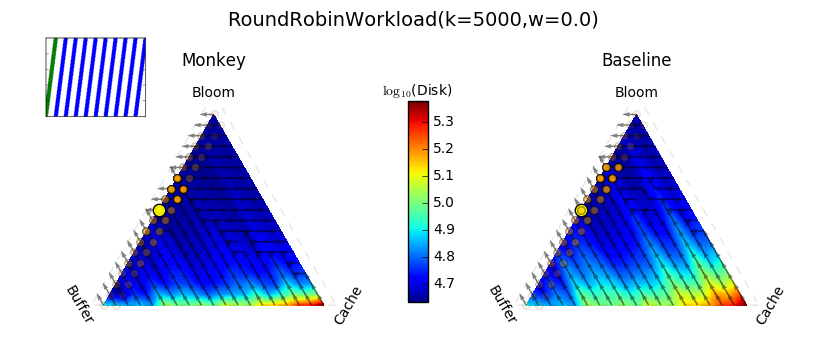
\includegraphics[width=0.5\textwidth]{robinquiv1.png}
\end{center}
\caption{Uniform and Round-Robin simulation results overlaid with gradient
    estimates.}
\label{fig:basicquiv}
\end{figure}


\begin{figure}[!htb]
\begin{center}
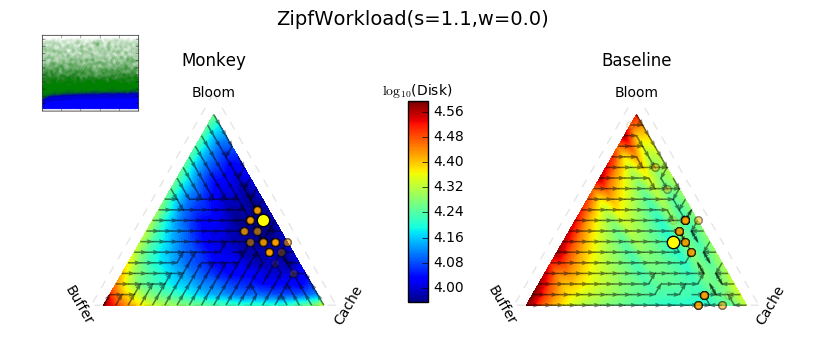
\includegraphics[width=0.5\textwidth]{zipfquiv1.png}
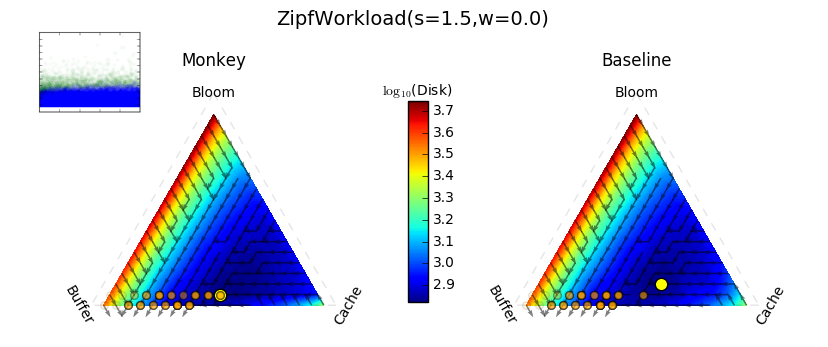
\includegraphics[width=0.5\textwidth]{zipfquiv2.png}
\end{center}
\caption{Zipf simulation results overlaid with gradient estimates for $s=1.1$
(lightly skewed) and $s=1.5$ (highly skewed).}
\label{fig:zipfquiv}
\end{figure}

The results for Zipf workloads in Figure \ref{fig:zipfquiv} look quite
different. At high skewness $s$, we find that Bloom filters are less useful and
it is better to allocate more memory to the buffer. At low skewness, the best
configuration is a mixture of mostly Bloom filter and cache memory with a
relatively small buffer.

This effect may be due to the fact for highly skewed workloads, we obtain
better savings for the small hot set of keys by using the cache (for reads) and
the buffer (for writes, and also as kind of auxiliary cache). For less skewed
workloads, we are more likely to request unpopular keys which may be buried
deep in the tree and impose a very high IO cost. To counteract this, we need
better Bloom filters.

\begin{figure}[!htb]
\begin{center}
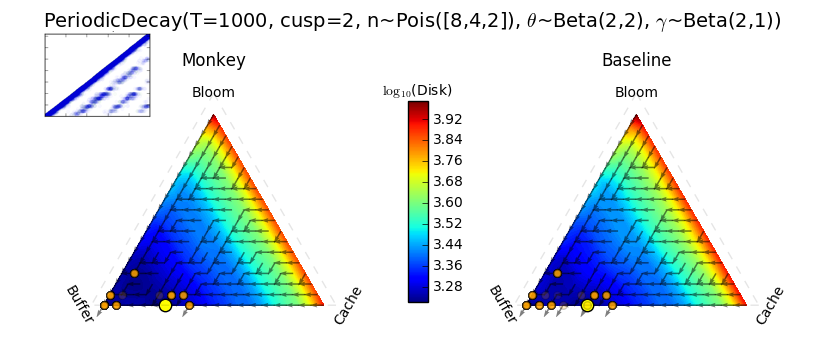
\includegraphics[width=0.5\textwidth]{periodquiv3.png}
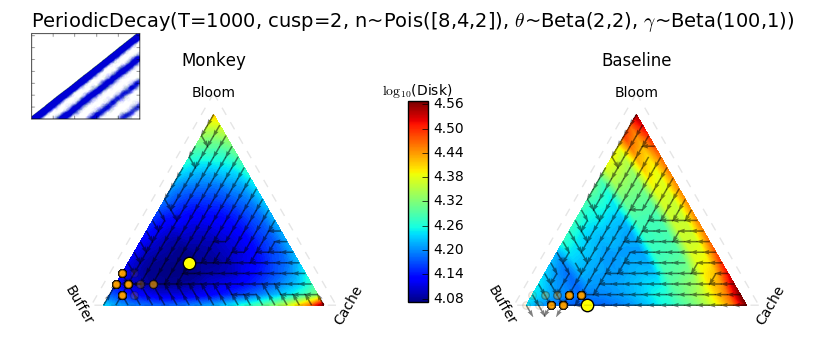
\includegraphics[width=0.5\textwidth]{periodquiv2.png}
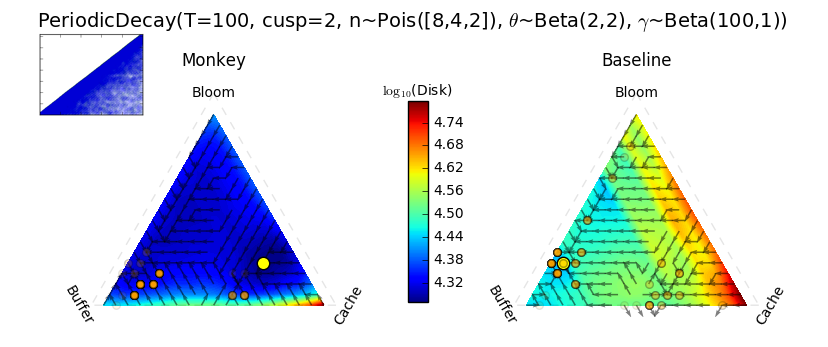
\includegraphics[width=0.5\textwidth]{periodquiv1.png}
\end{center}
\caption{Periodic Decay.}
\label{fig:periodquiv}
\end{figure}

Finally, for the Periodic Decay workloads, we find that our gradients
capture the behavior we noted near the beginning of the paper. For lower
effective numbers of popular keys (but high temporal locality), we tend
to end up allocating most of our memory to the buffer and none to the bloom
filters, but as our ``working set'' expands, we are pushed closer to the center
of the graph. In the bottom row, gradient descent is drawn into two distinct
modes based on the starting location, suggesting that our gradient estimations
are high-resolution enough to capture the nonconvexity. In general, there are
many situations in which increasing either the buffer or the bloom filter will
reduce I/Os, so we should expect multiple locally optimal allocation strategies
to exist.

For the complete set of results, please see Appendix \ref{fullresults}.

\clearpage

\bibliography{bibliography}
\clearpage

\appendix

\section{Benchmark workloads} \label{workloads}

\begin{figure*}[!h]
\centering
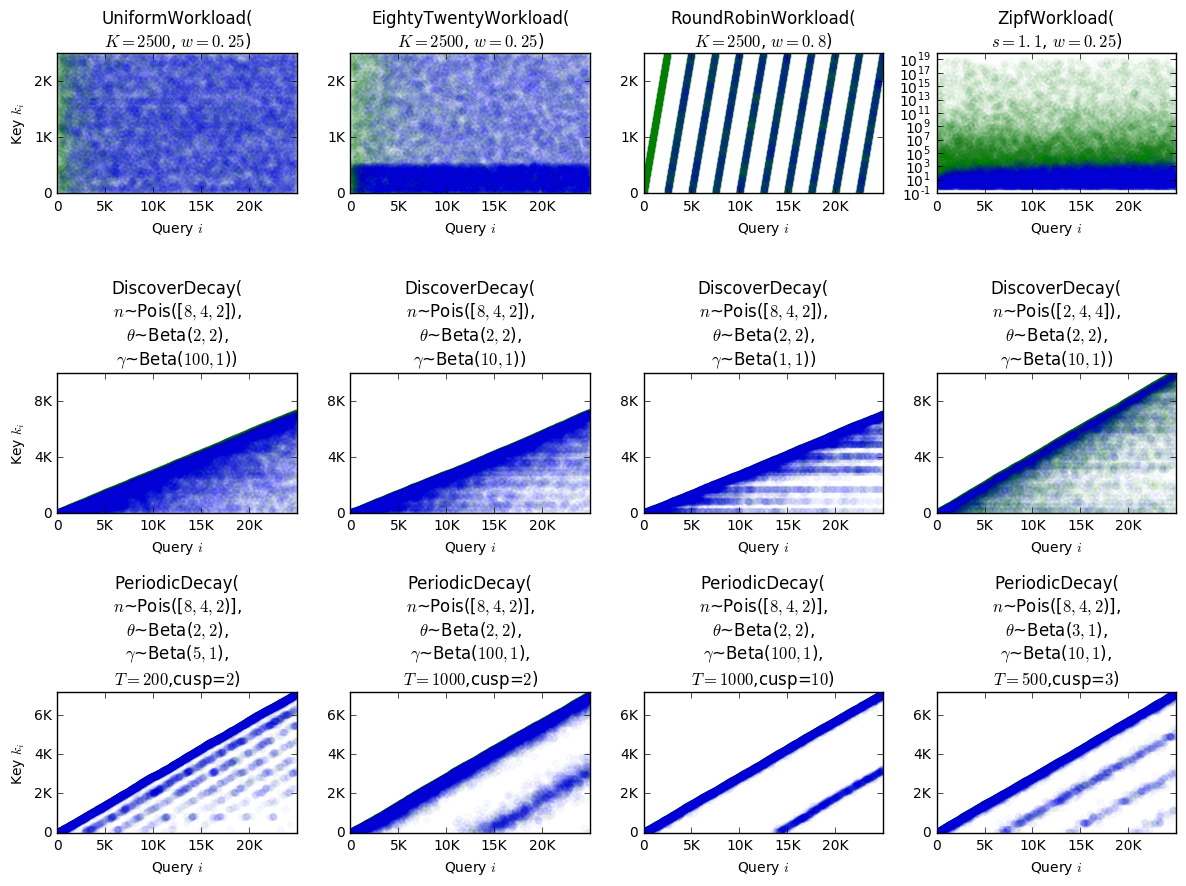
\includegraphics[width=0.80\textwidth]{workloads.png}
\caption{Example workloads we generated for benchmarking. The first row
  contains simple workloads where the distribution of key popularities does not
  change over time, and where the read/write ratio is a uniform probability.
  The second row contains Discover-Decay workloads, which add/read/update keys
  according to Poisson processes and simulate popularity decays over time. The
  third row is a modified version of Discover-Decay that adds a periodic signal
  to the decaying popularity with a configurable period and cusp sharpness. Blue
  dots represent reads and green dots represent writes or updates.}
\label{fig:workloads}
\end{figure*}

\clearpage

\section{Modeling} \label{modeling}

We first consider the case of a uniform query distribution and then show how
the formulation can be generalized to any distribution with an empirical trace.

\subsection{Uniform query distribution}

\noindent Assuming we have
\begin{itemize}
\itemsep-1em
\item $N$ items in total DB \\
\item $E$ size of an entry in bits \\
\item $M$ total memory \\
\item $M_c$ memory allocated to cache \\
\item $M_b$ memory allocated to buffer\\
\item $B$ entries that fit in a disk page \\
\item $P_b$ size of the buffer in pages, i.e. $\frac{M_b}{BE}$ \\
\item $T$ ratio between layers of LSM tree such that \\
\item $L1 = T * P_b * B$, $L2 =T^2 * P_b*B $, and so on,
\end{itemize}

\noindent then we can solve for $L$ the total number of layers required to store all the data: \\
$$P_b*B * \frac{1-T^L}{1-T} = N$$
$$L= \lceil \textrm{log}_{T} \left(\frac{N(T-1)}{BP_b} + 1\right) \rceil$$


The average cost of a write remains the same as for the basic LSM tree case:

$$
\text{write cost} = \textrm{log}_{T} \frac{N}{P_bB}
$$

The average cost of a read must be considered probabilistically over all
possible locations of the read item, in this case assuming a uniformly random
distribution of reads:

\begin{itemize}
\item Probability that read is in buffer $= p(\text{MT}) = \frac{P_b*B}{N}$
\item Probability that read is in cache $= p(\text{cache}) = \frac{M_c/E}{N}$
\item Probability that read is in L1 but not in cache $= p(L1)$ $$= \frac{P_b*B * T - \frac{P_b*B*T}{N-P_b*B} * M_c/E}{N}$$
\end{itemize}

where the numerator is the number of items $P_b*B*T$ that are in the first layer
minus the proportion of items from that layer that are probabilistically in the
cache already: $$\frac{P_b*B*T}{N-P_b*B} * M_c/E$$ and finally where the $N-P_b*B$
comes from the fact that items already in buffer (L0) are not allowed to
occupy the cache.

Therefore, given a uniform query distribution, the full expected cost in disk
reads of a read is
$$E[C_{\text{uniform}}] = p(\text{MT}) * 0  + p(\text{cache}) * 0 + \sum_{i=1}^L p(L_i) * i$$
$$=\sum_{i=1}^L \frac{P_b*B * T^i - \frac{P_b*B*T^i}{N-P_b*B} * M_c/E}{N} * i$$


\subsection{Bloom Filters}

The previous analysis hasn't yet accounted for the presence of Bloom filters,
which reduce the likelihood we will unnecessarily access a lower layer. For a
Bloom filter of $k$ bits with $h$ independent hash functions $h_1, h_2,...h_h$,
the probability that a given bit is still set to 0 after inserting $n$ keys is 

$$
(1 - \frac{1}{k})^{n*h}
$$
Then the probability of a false positive is 
$$
(1- (1 - \frac{1}{k})^{n*h})^h \approx (1 - e^{-hn/k})^h
$$

We can minimize this over $h$ to find the optimal number of hash functions,
which is $h = \mathrm{ln}(2) * \frac{k}{n}$. Assuming that this is the number
of hash functions $h$ we will use, the probability of a false positive as a
function of the number of bits is then 

$$
(1 - e^{-\mathrm{ln}(2)*k/n*n/k})^{\mathrm{ln}(2) * \frac{k}{n}} = (\frac{1}{2}) ^ {\mathrm{ln}(2) * \frac{k}{n}} \approx (.6185) ^  {\frac{k}{n}}
$$

For an item in any any level $L_i$ of the LSM tree with $i \geq 2$ we can
reduce the expected cost of accessing that item from $i$ by the number of Bloom
filter negatives at any level $j<i$. \\ \\ Then the expected cost of accessing
an item at $L_i$ is  $$\sum_{j=1}^{i-1} p(fp_j) * 1 + 1$$ Where $p(fp_j)$ is
the probability of a false positive for that key at level $j$ and 1 is the cost
of actually accessing the item at level $i$ assuming fence pointers that lead
us to the correct page.

\subsection{Expected Cost with Bloom Filters - Base Case}

Assuming a random distribution of reads, we now consider also the probability that a bloom filter allows us to ignore a level: \\
Expected cost of read for an item in the tree = $$p(mt) * 0  + p(cache) + 0 + \sum_{i=1}^L p(Li) * \sum_{j=1}^{i-1} p(fp_j)$$ \\
Expected cost for a null result read = $\sum_{j=1}^{L} p(fp_j)$

Given a total memory allocation $M$, the total number of bits we can allocate
to bloom filters is $M-M_c = \sum_{i=1}^L m_i$ \\ Then the total formula for
the expected cost of a read in the tree is: 

\begin{multline}
$$E[c] = \sum_{i=1}^{L} \frac{B*P*T^i - \frac{P_b*B*T^i}{N-P_b*B} * M_c/E}{N} \\ \cdot \left[ \left(\sum_{j=1}^{i-1} (.6185) ^  {\frac{m_j}{P_b*B*T^j}}\right) +1 \right]$$ 
\end{multline}

Whereas with a given percentage of null reads in the workload $p_{null}$:

\begin{multline}
$$E[c] = (1-p_{null})\sum_{i=1}^{L} \frac{P_b*B*T^i - \frac{P_b*B*T^i}{N-P_b*B} * M_c/E}{N} \\ \cdot \left[ \left(\sum_{j=1}^{i-1} (.6185) ^  {\frac{m_j}{P_b*B*T^j}}\right) +1 \right] + p_{null}\sum_{j=1}^{L} p(fp_j)$$
\end{multline}
\begin{multline}
$$E[c] = \sum_{i=1}^{L} (1-p_{null})\frac{P_b*B*T^i - \frac{P_b*B*T^i}{N-P_b*B} * M_c/E}{N} \\ \cdot \left[ \left(\sum_{j=1}^{i-1} (.6185) ^  {\frac{m_j}{P_b*B*T^j}}\right) +1 \right] + p_{null} \cdot p(fp_i) $$
\end{multline}

\subsection{Gradients of Cost with Bloom Filters - Generalized Distribution}

\subsubsection{Cache Gradient}

Note that in the above, the workload specific factors are the probability that
a read is at any given level and the related probability that any given item
from a level is already in the cache. To compute an empirical estimation of the
probability that any given item is in a layer but not already in the cache, we
can simply keep statistics on the total number of times a key was found in that
layer divided by the total number of (non-null) read queries executed. Then we
can consider the following simplification:

\begin{multline}
$$E[c] = \sum_{i=1}^{L} (1-p_{null})\left[p(L_i) - \frac{p(L_i)}{(N - P_bB)} * M_c/E \right]\\ \cdot \left[ \left(\sum_{j=1}^{i-1} (.6185) ^  {\frac{m_j}{P_b*B*T^j}}\right) +1 \right] + p_{null} \cdot p(fp_i) $$
\end{multline}

Taking the derivative with respect to the number of entries in the cache,
$M_c/E$, we get:

$$
\sum_{i=1}^{L}  -(1-p_{null}) p(L_i)/(N - P_bB) \cdot \left[ \left(\sum_{j=1}^{i-1} (.6185) ^  {\frac{m_j}{P_b*B*T^j}}\right) +1 \right]
$$

Which is just the average cost of a read throughout the tree. Then, to keep
statistics on how valuable we expect the cache to be, we maintain statistics on
the average cost of every read performed in the window of interest.

\subsubsection{Bloom Filter Gradients}

Because the memory allocation problem is discrete anyway, we consider the value
of the bloom filters as a finite difference, that is the approximate value of
any marginal bloom filter bit at layer $k$ will be $E[c | m_k+1] - E[c | m_k]$.
In this computation, all terms in the sums drop out except for those concerning
$m_j$, and we are left with:

\begin{multline}
$$\sum_{i=k}^{L} (1-p_{null})\left[p(L_i) - \frac{p(L_i)}{(N - P_bB)} * M_c/E \right] \\ \cdot \left\{ \left[ \left( (.6185) ^  {\frac{m_k+1}{P_b*B*T^j}}\right) +1 \right] - \left[ \left( (.6185) ^  {\frac{m_k}{P_b*B*T^j}}\right) +1 \right] \right\} \\+ p_{null}  \left( (.6185) ^  {\frac{m_k+1}{P_b*B*T^j}} - (.6185) ^  {\frac{m_k}{P_b*B*T^j}}\right)$$
\end{multline}

Rearranging terms, we get:
\begin{multline}
$$\sum_{i=k}^{L} \left[(1-p_{null})\left[p(L_i) - \frac{p(L_i)}{(N - P_bB)} * M_c/E \right] +  p_{null} \right] \\ \cdot \left( (.6185) ^  {\frac{m_k+1}{P_b*B*T^j}} - (.6185) ^  {\frac{m_k}{P_b*B*T^j}}\right)$$
\end{multline}

Where this is exactly the number of times the given bloom filter is accessed
times the difference in the theoretical false positive rates given memory
allocations $m_j$ and $m_j+1$. Then, to keep statistics on how valuable we
expect any given bloom filter to be, we maintain statistics on the number of
times every bloom filter was accessed in the window of interest.

\subsubsection{Buffer Gradient: Gets}

To estimate the additional value of any marginal memory in the buffer with
respect to reads, we must make a number of simplifications, as $P_b$, the number
of pages in the buffer, factors into every term in this equation. Further, the
interaction between $P_b$ and most of the terms is not available in closed form,
in general. Rather, the critical terms $P(L_i)$ we are empirically estimating.
Then, for reasonably large values of $N$ and $P_b$, we will assume that the bloom
filter false positive rate stays approximately the same, as does the value of
the cache. Then, we consider only the change in I/Os occurring from the altered
probability of any given element occurring in any layer as a result of more
elements being in the buffer. We can provide a simple estimate
of this by assuming that any items we add to the buffer would have
otherwise occurred in L1, and in the resulting cascade, $T^{i}$ times that number of items will be moved up into 
each layer $L_{i}$ from the layer below.

Then, an appropriate estimate of how useful any additional space of memory in
the buffer is for reads is simply the resulting change in $p(L_i)$ for each layer (that is, the number of hits
we expect to see on the newly added elements) $* fp_{i}$ for any layer $i\neq0$, as the original cost of accessing that element was $\sum_{j=1}^i fp_{j} + 1$, and the new cost of accessing is $\sum_{j=1}^{i-1} fp_{j} $, the difference between which is just $fp_{i}$. For $i=0$, the buffer itself, the expected savings per hits is exactly 1, as the item will be moved from having an access cost of 1 to 0. To estimate how many additional times L1 would be accessed if
we instead allocated the final portion of the buffer to L1, we keep
statistics on how often the final spots of the buffer were accessed in a
read. In practice, these spots are accessed only very infrequently, as the
buffer is accessed only a handful of times at this stage before being flushed.
This statistic might be more helpful on a system with constant compaction
rather than a full layer flush. For the rest of the layers, we simply assume the same hit rate per key
as measured over the existing keys on any level and multiply by the number of elements we will be adding to calculate
the expected accesses to the new keys on each level. We then multiply by the empirical rate of bloom filter false positives on the level.

\subsubsection{Buffer Gradient: Puts}

For the buffer, we must additionally consider the saved update/insert I/Os.  $$
\text{write cost} = \textrm{log}_{T} \frac{N}{P_bB} $$ Taking the derivative with
respect to $P_bB$, the number of items in the buffer, we get $\frac{1}{P_bB}$ In
discrete terms, this evaluates to $\textrm{log}_{T} \frac{P_bB}{P_bB+1}$. 

Unfortunately, this simplification only works if we can assume that memory is being allocated in 
page-size chunks and that the workload has no duplicates. In practice, the number of I/Os associated
with reading and writing throughout the merging process is a stepwise function that depends on page size, as reading or
writing one element from or to a page has the same I/O cost as reading or writing a full page. To simplify our analysis
of the page size write savings, we consider only a ratio of $T=2$, and we begin by addressing the case wth no 
duplicates. 

With no duplicates, the final number of elements at any level of the tree is a
deterministic function of the number of elements inserted as well as the layer
sizes. Then considering the empirical number of items inserted into the buffer
as well as the size of the original buffer, we can solve for the theoretical
final structure of an alternate LSM tree that had a buffer of size $P_bB + 1$.

Additionally, given the number of elements on any given layer, no duplicates,
and an original buffer size $P_bB+1$, we know the number of times each
$T^{i}*(P_bB+1)$-size chunk on each level will have been read and written given
the current fullness of the layer. We can then multiply these numbers of known
chunk reads and writes by the ceiling of the size of those possible chunks
(which, with ratio $T=2$ will be $T^{i}*(P_bB+1)$ and $T^{i}*(P_bB+1)*2$) divided
by pagesize, $B$. This gives us a more realistic number in which additions of
less than a pagesize of memory are not helpful in I/O savings. 

Comparing the read and write costs of this theoretical tree to the empirical
reads and writes accesses of the existing tree gives us an expected I/O savings
related to updates for the larger tree.

We consider additionally the fact that I/O savings are in general lessened by
the number of duplicates inserted, as duplicates will not be merged the full
length of the tree. To take this into account we also keep a statistic for the
total number of duplicates merged over the window of interest per layer and use
this to calculate the percentage of duplicates removed relative to total keys
at each level. This factors in in several places. First, when computing the
theoretical allocation of keys in the final tree, we consider the total number
of items that would have come in to the buffer from the empirical
count and adjust this at each layer by the percentage that are expected to have
been removed as duplicates. Further, when computing read and write I/Os during
merging, we expect that number of items written when the layer is already half
full should be decreased by the expected number of duplicates removed among the
two sets of keys. Again, the resulting I/O savings will be stepwise in
pagesize. In particular, if the original size of the array would have only been
slightly into the final page, it will take very few duplicates to reduce the
I/O count by 1, whereas if all pages would have been full, it will take a full
page's worth of duplicate removals to improve I/Os. The same savings will be
experienced again when these items are read to be merged into the lower layer.

The correct way to handle the duplicates requires somewhat more consideration,
but the only statistics we are currently using The are the empirical number of
update queries and the empirical number of duplicates found and removed on each
layer over the window of interest.


\subsection{Estimating Statistics with $O(1)$ Memory}

\textbf{Cache:} to estimate the number of disk accesses we will save by adding
$dM$ extra bits of memory to the cache, we let consider $dM$ as a number of
extra entries in the cache. That is, we calculate the savings from having
$dM/E$ extra cache entries available. As mentioned above, the relevant
statistic here is the average cost of a read in the database. To calculate
this, we collect statistics on the total number of disk accesses and total
number of queries. The expected cost per query is then the number of disk
accesses over the window divided by the total number of queries. To approximate
the probability of the item being in the cache times the number of queries, we
maintain a statistic for the number of times the last cache slot was accessed
during the window of interest and make the assumption that the number of hits
on the next marginal slot(s) would be approximately the same. Then we can
calculate the final expected I/O savings as

$$dM/E * E[hits] * E[cost/query]$$

\textbf{Bloom Filters:} To estimate the number of disk accesses we will save by adding $dM$ extra bits of memory to the bloom filters, we first decide how to allocate that $M'_{bloom} = M_{bloom}+dM$ bits using Monkey or the baseline allocation, giving us $m_i$ and $m'_i$ bits per bloom filter on each layer. At each layer $i$, for both $m_i$ and $m'_i$, we update rolling averages of the theoretical false positive rate $\hat{fp}_i = \mathbb{E}\left[0.6185^{\frac{m_i}{n_i}}\right]$ and $\hat{fp}'_i = \mathbb{E}\left[0.6185^{\frac{m'_i}{n_i}}\right]$ every time the bloom filter is queried (where $n_i$ is constantly changing based on insertions and flushes of the filter). These statistics (individual floats) give us an estimate of the aggregate false positive rate at $m_i$ and $m'_i$ robust to changing layer fullness. Finally, we keep a counter $n_{i,\text{bloom false}}$ of the number of times requested items are \textit{not} in bloom filter $i$. This counter is incremented either when the bloom filter returns false (which we know immediately) or returns a false positive (which we can record after fruitlessly searching the layer). This counter allows us to estimate disk accesses resulting from our current or altered false positive rates. The final savings is therefore \[
  \text{Savings}(M'_{bloom}) = \sum_{i} (\hat{fp}'_i - \hat{fp}_i) * n_{i,\text{bloom false}},
\]

and only requires keeping two floats and one integer. Note that in our simulation, for flexibility, we keep a histogram of $n_i$ values at each bloom filter request to avoid needing to predetermine $m'_i$, but in a practical implementation this is unnecessary.

Note that because we can obtain these estimates on a layer-by-layer basis, we can investigate whether reallocating memory from one bloom filter to another, empirically, should reduce I/Os. Validating the results of Monkey \cite{monkey}, in Figure \ref{fig:bloom-realloc} we find that for the baseline allocation, moving bits does improve performance, but for Monkey, it does not, regardless of workload.

\begin{figure}[!htb]
\begin{center}
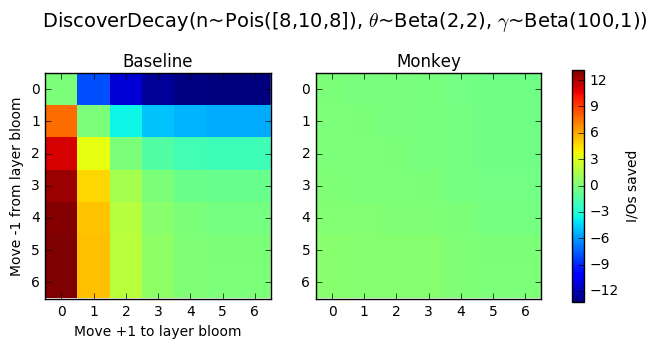
\includegraphics[width=0.33\textwidth]{bloom-moves-disc.png}
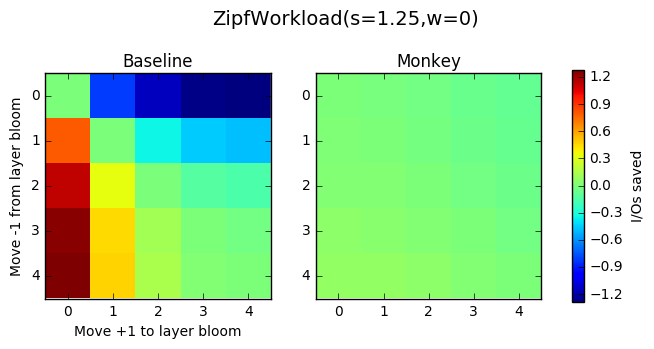
\includegraphics[width=0.33\textwidth]{bloom-moves-zipf.png}
\end{center}
\caption{Estimated change in I/Os when moving bits from one bloom filter to another (keeping total bloom filter memory constant). Regardless of workload, changes in I/Os for Monkey are all less than 1, indicating its optimality.}
\label{fig:bloom-realloc}
\end{figure}

\textbf{Buffer:} To estimate the number of disk accesses we will save in reads by adding $dM$ extra bits of memory to the buffer, we use statistics maintained on the total bloom filter accesses per layer, bloom filter false positives per layer, and hits per layer. We estimate the expected
additional number of hits on any given layer as the original hits times the new theoretical size divided by the actual original size.
That is, the number of extra hits is equal to $$new\_hits_{i} = hits_{i} * \frac{size_{i} + dM*T^{i} }{ size_{i}}$$
For each expected hit, we have an I/O savings equal to the false positive rate on the bloom filter of that layer, as described in the previous section. To calculate this for a layer $i$, we use 
$$E[savings/hit]_{I} = \frac{false\_positives_{i}}{bloom\_accesses_{i}}$$
Then the total number of I/Os saved should be 
$$
\sum_{i=0}^L new\_hits_{i} * E[savings/hit]_{i} 
$$
where for layer 0, the buffer, the $E[savings/hit] = 1$, as the access cost at L1 is always exactly 1 and the access cost at 
the buffer is always 0.

To estimate the number of disk accesses we will save in writes/updates by adding $dM$ extra bits of memory to the buffer, 
we maintain statistics on total number of entries that passed through any given layer, number of duplicates removed at any given layer, and number of entries in any given layer at the end of the period. For a workload without duplicates, we can simply
use these statistics to deterministically calculate the final allocation and number of read and write I/Os that would have
occurred throughout the process for a second tree with buffer size + $dM$, calculating every batch of read and write merges and summing over the number of pages that would have been involved. For the original tree we can either use statistics on empirical I/Os during the merging process or use the same deterministic formula to calculate what they would have been. The expected saved I/Os then is simply

$$cost_{tree} - cost_{tree+dM}$$

When we consider duplicates, the estimate becomes much more noisy. To consider the effect of duplicates on reducing the total number of pages read and written during the merging process, we reduce the number of entries that pass through each layer of our theoretical larger tree by the percentage of duplicates removed at each layer, calculated as $$\frac{duplicates\_removed_{i}}{total\_entries_{i}}$$

This then changes the final layer structure of the estimated tree. We also consider that duplicates should reduce the total number of entries written and then read after two segments are merged together. Then for those read and write components that occur on an already half-filled layer, we reduce the number of elements by multiplying by $$1 - \frac{duplicates\_removed_{i}}{total\_entries_{i}}$$
This will reduce the total I/Os by number of page reads it makes unnecessary. With this adjusted cost for the larger tree, we again calculate the expected saved I/Os as the estimated I/Os of the hypothetical larger tree subtracted from the empirical or theoretical I/Os of the existing tree.

\subsection{Testing Accuracy and Variance of Statistics}

To confirm that our estimates are reasonable, we ran 250 simulations for three
separate workloads and compared our estimates of each gradient to the actual
savings for a separate tree with 8 bytes of extra memory in the corresponding
LSM component (against which we ran the same workload). Results can be seen in
Figure \ref{fig:savings}.

There is a large amount of variance in the simulated results, both because of
randomness in the separate instantiations of the workload and randomness in
the execution of its queries, but for the most part, our estimates of the average
savings are both precise and accurate. There is a slight deviation for the uniform
buffer savings calculation, but the variance is so high that it does not appear
to be significant.

The fact that our estimates of the expected I/O savings are so precise across
workloads gives us confidence first that our simulation and modeling are correct,
and second that they will generalize to more complex, real-world workloads
with more queries and keys.

\begin{figure*}[!htb]
\centering
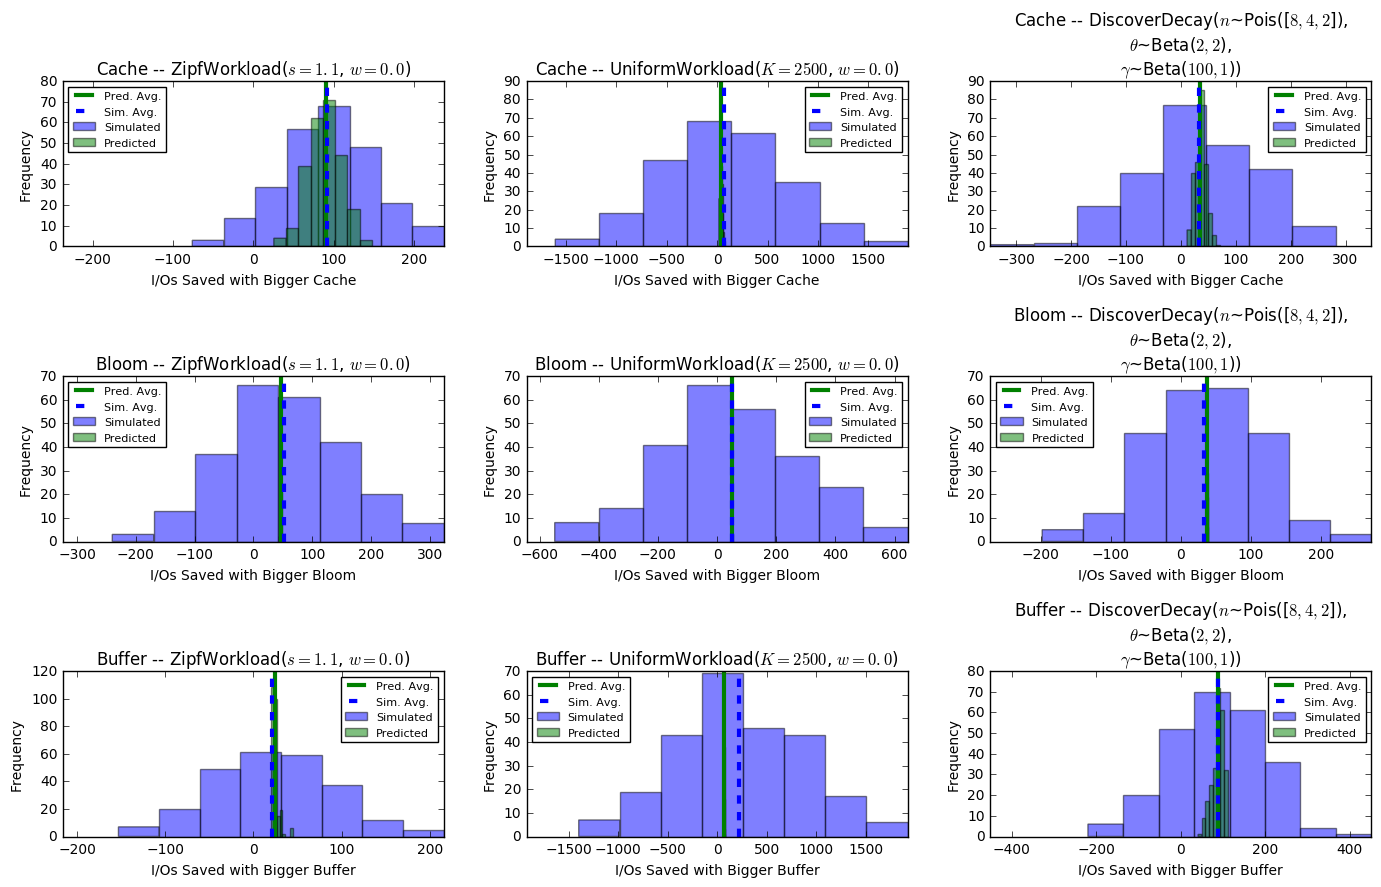
\includegraphics[width=0.8\textwidth]{all-savings.png}
\caption{Light-footprint statistical estimations of the gradient vs. simulated
results for cache, bloom filters, and the buffer on three distinct workloads.}
\label{fig:savings}
\end{figure*}


\clearpage

\section{Full Results} \label{fullresults}

\begin{figure}[!htb]
\begin{center}
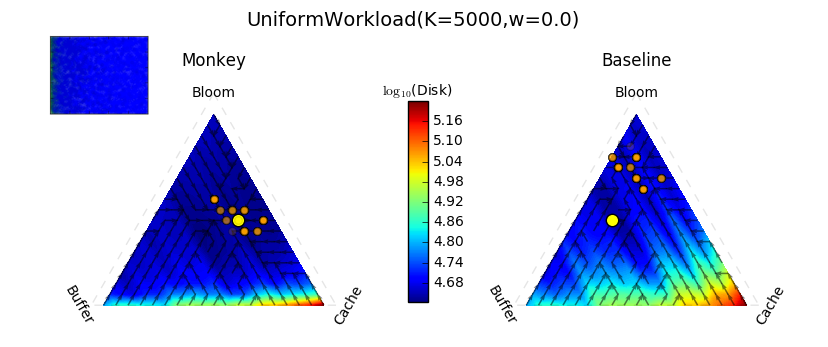
\includegraphics[width=0.5\textwidth]{uniformquiv1.png}
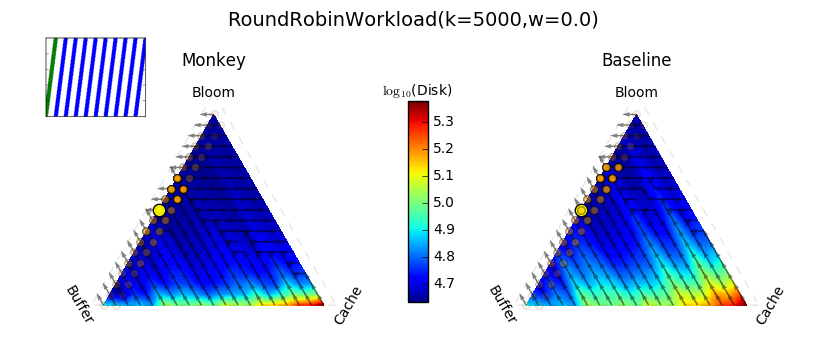
\includegraphics[width=0.5\textwidth]{robinquiv1.png}
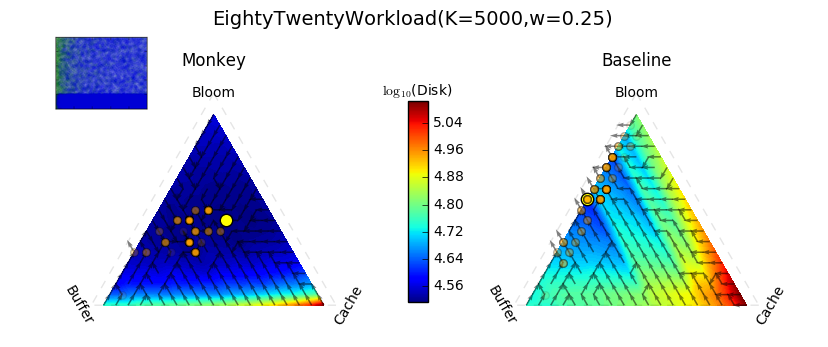
\includegraphics[width=0.5\textwidth]{eightwenquiv2.png}
\end{center}
\caption{Basic workload simulation results.}
\end{figure}

\begin{figure}[!htb]
\begin{center}
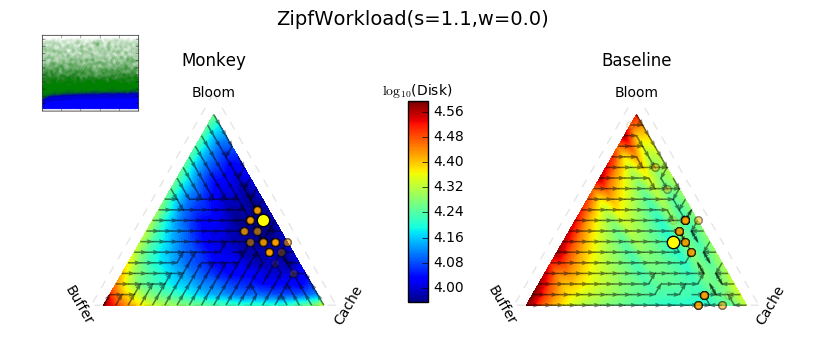
\includegraphics[width=0.5\textwidth]{zipfquiv1.png}
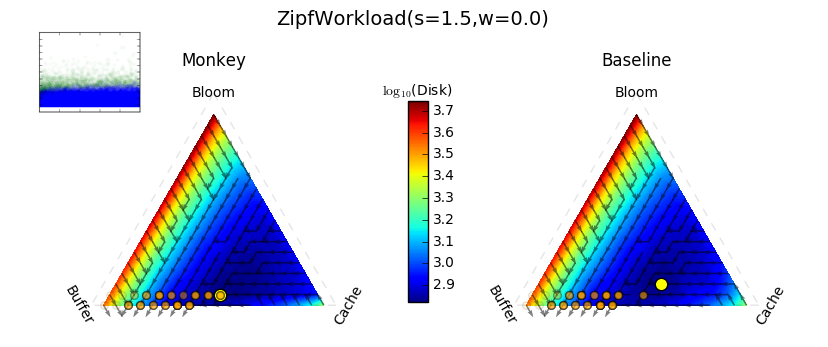
\includegraphics[width=0.5\textwidth]{zipfquiv2.png}
\end{center}
\caption{Zipf simulation results overlaid with gradient estimates for lightly skewed and highly skewed.}
\end{figure}

\begin{figure}[!htb]
\begin{center}
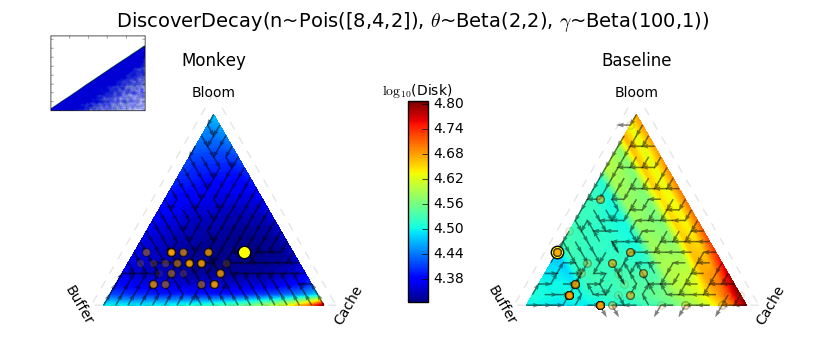
\includegraphics[width=0.5\textwidth]{discdecquiv2.png}
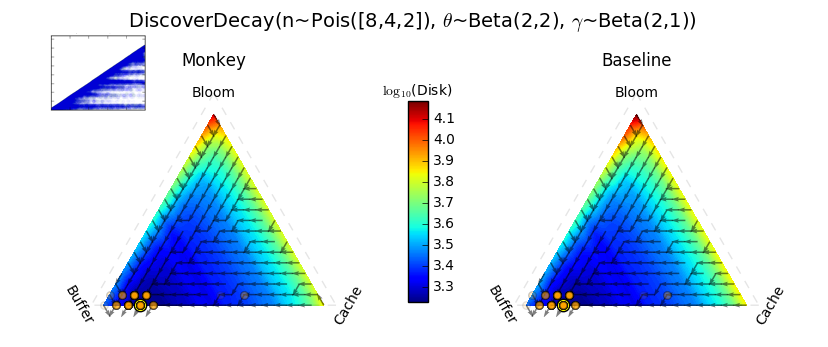
\includegraphics[width=0.5\textwidth]{discdecquiv1.png}
\end{center}
\caption{Discover-Decay simulation results overlaid with gradient estimates for
    lightly skewed and highly skewed.}
\end{figure}

\begin{figure}[!htb]
\begin{center}
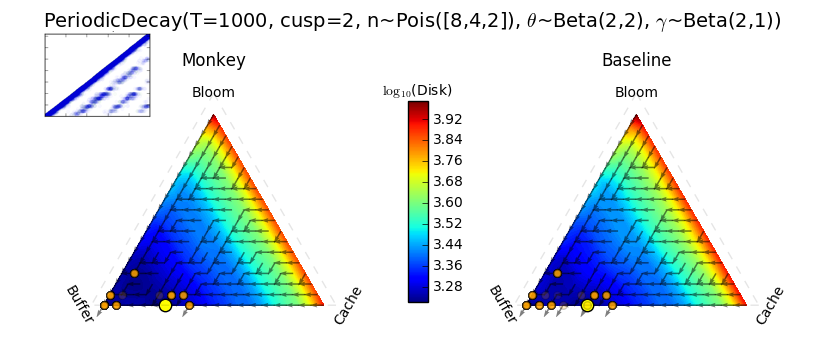
\includegraphics[width=0.5\textwidth]{periodquiv3.png}
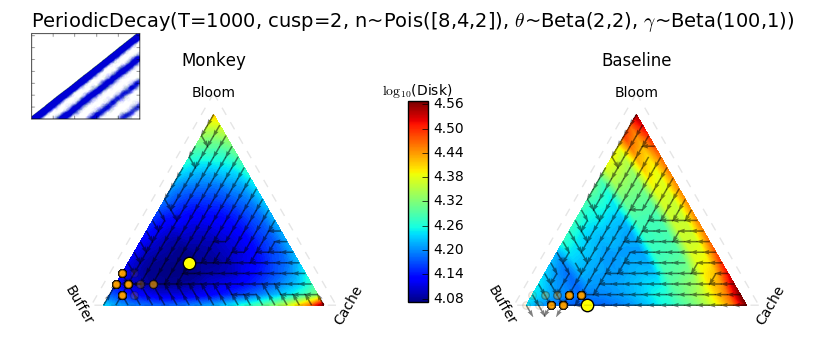
\includegraphics[width=0.5\textwidth]{periodquiv2.png}
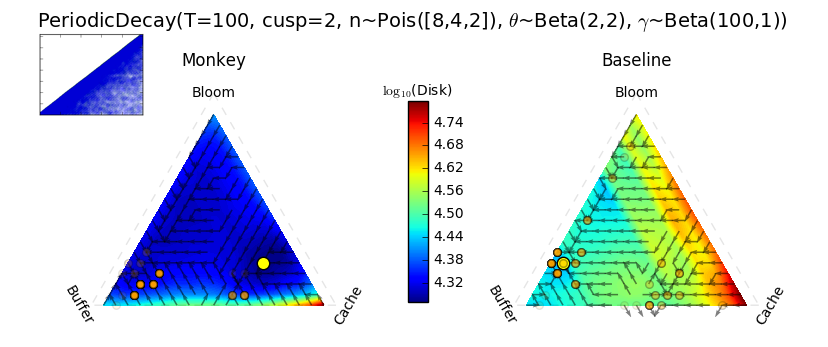
\includegraphics[width=0.5\textwidth]{periodquiv1.png}
\end{center}
\caption{Periodic Decay simulation results.}
\end{figure}

\end{document}
